\documentclass[conference]{IEEEtran}
\IEEEoverridecommandlockouts
% The preceding line is only needed to identify funding in the first footnote. If that is unneeded, please comment it out.
\usepackage{cite}
\usepackage[portuges,brazil,english]{babel}
\usepackage{amsmath,amssymb,amsfonts}
\usepackage{algorithmic}
\usepackage{graphicx}
\usepackage{textcomp}
\usepackage[export]{adjustbox}
\usepackage{float}
\usepackage[ruled,vlined,linesnumbered,portuguese]{algorithm2e}
\usepackage[utf8]{inputenc}
\def\BibTeX{{\rm B\kern-.05em{\sc i\kern-.025em b}\kern-.08em
    T\kern-.1667em\lower.7ex\hbox{E}\kern-.125emX}}
\begin{document}

\title{Trabalho 3 - MC886 Aprendizado de Máquina}

\author{\IEEEauthorblockN{Leo Yuuki Omori Omi}
\IEEEauthorblockA{
138684 \\
leoyuuki@gmail.com}
\and
\IEEEauthorblockN{João Pedro Ramos Lopes}
\IEEEauthorblockA{
139546 \\
jpedrorl@gmail.com}}

\maketitle

\section{Introdução}

Neste trabalho, tivemos que agrupar vários textos utilizando utilizando técnicas de Aprendizado não-supervisionado. Utilizando dados em formato \textit{bag-of-words} utilizamos algumas técnicas para tentar achar agrupamentos que fizessem algum sentido.

\subsection{Soluções Propostas}

\subsubsection{DBSCAN}
Tentamos utilizar a técninca Density-Based Spatial Clustering of Applications with Noise (DBSCAN), já implementado na biblioteca Scikit Learn. Parecia uma boa escolha já que o algoritmo agrupa pontos próximos um dos outros, sem precisar receber como parâmetro o número de grupos (que é um dos resultados que gostaríamos). Tentamos variar os parâmetros \texit{eps} e \textit{min\_samples}, no entanto, inicialmente, não conseguimos achar uma configuração que desse um resultado que parecia coerente, portanto desistimos de continuar experimentos com esta técnica. Possivelmente, a distribuição dos dados não favorecia o DBSCAN ou mesmo foi uma escolha infortúnia do parêmtros.

\subsubsection{Hierarchical Clustering}
Foi utilizado a implementação de Hierarchical clustering da biblioteca SciPy para agrupar os textos utlizando a função fclusterdata. Ela recebe como parâmetros os dados, uma limiar de distância máxima entre dois pontos, e um critério de comparação (neste caso foi utilizada a distância). Assim como o DBSCAN, o número de grupos não é uma das entradas para a função, e o algoritmo trata de achar estes grupos.

\subsubsection{K-means}


\subsection{Experimentos}
Para todos os experimentos foi utilizado o Silhouette Coefficient como uma forma de avaliar a performance entre os métodos. 

\subsubsection{Modelos iniciais}
Para analisar o número de grupos presentes no problema, utilizamos como modelo base o Elbow Method, variando esse número no intervalo [10, 1000] com passo 10 encontramos o gráfico disposto na figura \ref{fig:elbow}. 

\begin{figure}[H]
  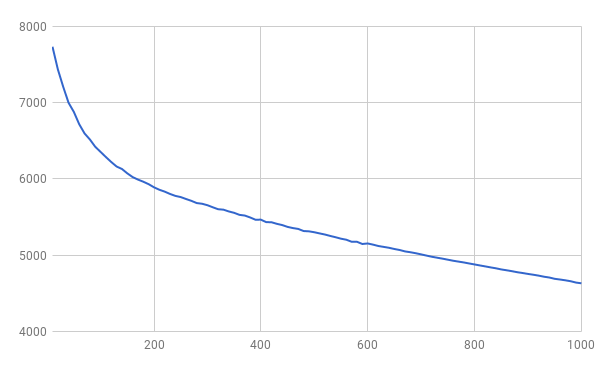
\includegraphics[scale=0.4, center]{elbow.png}
  \caption{Número de Clusters x Erro médio}
  \label{fig:elbow}
\end{figure}

Utilizando o modelo de k-médias com 3 reinícios, 10 iterações e inicialização aleatória \textit{k-means++}. Com base no gráfico gerado, escolhemos o range de classes [50, 400] a ser submetido ao método de silhueta. Utilizando passo 50 encontramos o gráfico da figura \ref{fig:sil1}, que representa a pontuação para tais valores de k.

\begin{figure}[H]
  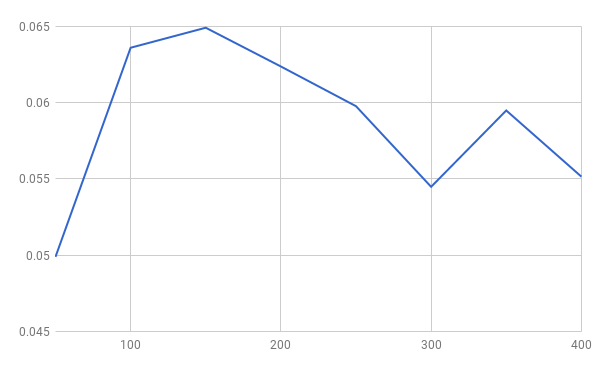
\includegraphics[scale=0.4, center]{silhouette1.png}
  \caption{Silhueta no intervalo [50, 400] com passo 50}
  \label{fig:sil1}
\end{figure}

Finalmente, para determinar o número de classes a ser utilizado pelo modelo, foi percorrido o intervalo [125, 175] e desenhado o gráfico da pontuação encontrada pelo método de silhueta, representado na figura \ref{fig:sil2}. Dessa forma, foram emscolhidas 151 clusters para o problema. 

\begin{figure}[H]
  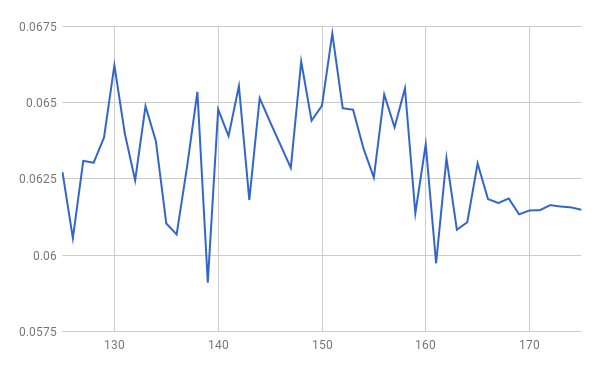
\includegraphics[scale=0.4, center]{silhouette2.png}
  \caption{Silhueta no intervalo [125, 175]}
  \label{fig:sil2}
\end{figure}

\subsubsection{Solução Base K-Means}
Para analisar o modelo final do k-means, utilizou-se a mesma configuração que anteriormente, com máximo de 300 iterações e $k=151$. Com estes parêmetros foi obtido um coeficiente de 0.067. Para checar os resultados encontrados, escolheu-se um agrupamento aleatório e ordenou-se os pontos pertencentes a ele pela distância euclideana. De forma amostral, checamos alguns clusters e percebemos que o assunto geral dos documentos mais próximos foram:

\begin{itemize}
\item Cluster 0: pedidos de ajuda e sugestões/dicas em diversos tópicos (carros, hardware
\item Cluster 17: discussões relacionadas a \textit{Hockey}
\item Cluster 31: 3 grupos principais: carros, esportes e eletrônicos
\item Cluster 42: Uma longa discussão sobre o mesmo assunto: \textit{Who's next? Mormons and Jews?}
\item Cluster 67: Questões relacionadas a hardware/software da Microsoft/Apple
\item Cluster 123: Alguns documentos são relacionados a vendas, outros relacionados a direção de veículos
\end{itemize}

\subsubsection{Hierarchical Clustering}
Foram `chutados`  alguns valores iniciais para o limiar do algoritmo. Assim, percebemos que valores menores que 1 estavam tendo um Silhoutte Coefficient melhor, portanto foi utilizado um laço para achar valores com melhores resultados. Foi utilizado metade do conjunto de dados por causa do tempo de execução longo. O coeficiente achado foi de 0.055 para o limiar de 0.7, assim, este valor foi utilizado.
No entanto, ao analisarmos melhor o resultado, foram criados mais 8500 grupos para as 9962 entradas de dados, ou seja, muitos dos grupos só possuiam um ponto. Analisando alguns dos clusters que tinham multiplos pontos, achamos coisas coerentes:

\begin{itemize}
\item Cluster 2: Placares e pontuações da MLB
\item Cluster 61: Accounts of Anti-Armenian Human Right Violations in Azerbaijan
\item Cluster 31: Venda de revistas Playboy do ex colega de quarto
\end{itemize}

Em clusters que possuem múltiplos pontos, encontramos texto muito parecidos ou iguais, o que podemos até considerar como mérito desta solução. No entanto, como ela forma um número enorme de grupos, esta solução não possui muita generalidade.

\section{PCA}
Considerando a solução do K-means como a melhor, aplicamos o PCA nos dados. Rodamos alguns testes usando os parâmetros achados e verificamos o Silhoutte Coefficient obtido para alguns valores de dimensionalidade do PCA. Segue uma tabela com alguns dos valores obtidos:

\begin{tabular}{ccc}
  \toprule[1.5pt]
  \head{Nº Componentes} & \head{Silhoutte} \\
  \midrule
  1000 & -0.0408837480849 \\
  500 & 0.0116988599587 \\
  250 & 0.0796884585275 \\
  100 & 0.15327313388 \\
  10 & 0.14025108712 \\
  \bottomrule[1.5pt]
\end{tabular}

Podemos ver que valores maiores das dimensões estão diminuindo o desempenho da solução de acordo com o Silhoutte Coefficient. No entando, conforme o número de dimensões no PCA foi diminuido, chegamos a um valor maior que o original, sendo que nos valores testados, obtemos o melhor resultado com 100 dimensões. Checando alguns clusters como foi feito anteriormente, encontramos novamente grupos com assunstos em comum.

No mínimo, conseguimos ganhar em desempenho computacional pois estamos rodando K-Means com um número menor de dados, assim demorando menos para treinar ou predizer valores.

\section{Conclusões}
Não ter uma `resposta correta` torna muito diferente e difícil a resolução de problemas. Aprendizado não-supervisionado requere mesmo uma análise do tipo de dado ou alguma técnica ou heurística para auxiliar na resolução dos problemas. No caso de nossos experimentos do K-Means, conseguimos achar um resultado coerente usando uma técnica conhecida, o Elbow Method. Sendo que DBSCAN, que parece que uma solução até mais robusta, nos trouxe dificuldades para calibrar seus parâmetros.

Não ter uma resposta exata para o problema também traz dificuldade para verificar o desempenho. Utilizamos o Silhoutte Coefficient e uma pequena checagem de alguns casos, mostrando alguns resultados bons.

\begin{thebibliography}{00}
\bibitem{linearregression1} Montgomery, D.C., Peck, E.A. and Vining, G.G., 2015. Introduction to linear regression analysis. John Wiley \& Sons.
\bibitem{gendreau2010handbook} Gendreau, M. and Potvin, J.Y., 2010. Handbook of metaheuristics (Vol. 2). New York: Springer.
\bibitem{continousgenetics} Haupt, R.L. and Haupt, S.E., 2004. Practical genetic algorithms. John Wiley \& Sons.
\bibitem{continuousgenetics2} Djurisic, A.B., Elazar, J.M. and Rakic, A.D., 1997. Genetic algorithms for continuous optimization problems-a concept of parameter-space size adjustment. Journal of Physics A: Mathematical and General, 30(22), p.7849.
\end{thebibliography}

\end{document}
